%   % !TEX root = ../../VIII,3_Rahmen-TeX_9-0.tex
%  
%   Band VIII, 3 N.~1?? 	[Stoß]
%   Signatur/Tex-Datei:	LH_37_05_162v
%   RK-Nr. 	57266_3		(_1 und _2 auf demselben Träger)
%   Titel: 			Mutationes celeritatum sint ut corpora concurrentia reciproce
%   Datierung:		März bis Mai 1677		
%   edlabels:			12	
%   Diagramme: 		5 (davon Fig. 1a/b zwei Fassungen, Fig. 2 gestr.)
%
%
%
\selectlanguage{ngerman}
\frenchspacing
%
\begin{ledgroupsized}[r]{120mm}
\footnotesize
\pstart
\noindent\textbf{Überlieferung:}
\pend
\end{ledgroupsized}
%
\begin{ledgroupsized}[r]{114mm}
\footnotesize
\pstart \parindent -6mm
\makebox[6mm][l]{\textit{L}}%
Konzept: LH~XXXVII~5, Bl.~162.
Ein~Blatt~2\textsuperscript{o};
Papierschaden an den Rändern mit geringfügigem Textverlust;
Papiererhaltungsmaßnahmen.
Eine Seite auf Bl.~162~v\textsuperscript{o};	
Bl.~162~r\textsuperscript{o} überliefert im oberen Bereich den Schlussteil von N.~\ref{57266_1} und
im unteren N.~\ref{57266_2}.
Vermutlich bildete der Träger ursprünglich einen Bogen mit LH~XXXVII~5, Bl.~161.
\pend
\end{ledgroupsized}
%
%
\selectlanguage{latin}
\frenchspacing
% \newpage%
\vspace{8mm}
\pstart%
\normalsize%
\noindent%
\edtext{%		Trick für A-Fn zu Diagramm
\edlabel{37_05_162v_11a}%
\lbrack162~v\textsuperscript{o}\rbrack %		
}{\lemma{}%
\Afootnote{\textit{Am Rand, oberhalb von \lbrack\textit{Fig.~2}\rbrack\ und \lbrack\textit{Fig.~3}\rbrack}: %
${\scriptstyle \textit{2}}P {\scriptstyle \textit{3}}P \,\sqcap P {\scriptstyle \textit{2}}P$ ob aequabilem motum centri.%
\protect\index{Sachverzeichnis}{motus aequabilis centri} Sit ${\scriptstyle \textit{2}}P {\scriptstyle \textit{3}}P \,\sqcap P$.%
\newline %
$\dfrac{{\scriptstyle \textit{3}}A {\scriptstyle \textit{3}}P}{{\scriptstyle \textit{3}}B {\scriptstyle \textit{3}}P}\,\sqcap \dfrac{\protect\ovalbox{\textit{b}}}{\protect\ovalbox{\textit{a}}}$. %
${\scriptstyle \textit{2}}A {\scriptstyle \textit{3}}A \smallfrown \protect\ovalbox{\textit{a}} + {\scriptstyle \textit{2}}B {\scriptstyle \textit{3}}B \smallfrown \protect\ovalbox{\textit{b}} \;\sqcap \langle e\rangle$ %
\lbrack\textit{Rechnung bricht ab}\rbrack%
}}
\pend%
\count\Bfootins=1100%
\count\Afootins=1100%
\count\Cfootins=1100
%
\pstart\noindent
\lbrack%
\textit{Erster Anlauf:}\rbrack 
\pend
%
\vspace{1.5em} %%%%%%%%% Diagramm 1a, erste Fassung
\centerline{%
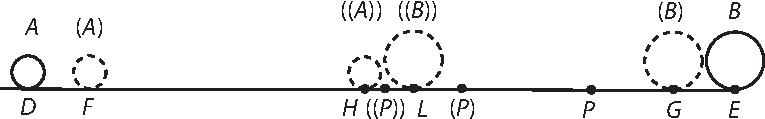
\includegraphics[width=0.66\textwidth]{%
gesamttex/edit_VIII,3/images/LH_37_05_162v_d1a.pdf%
}} 
\vspace{0.5em}
\centerline{%
\lbrack\textit{Fig.~1a, erste Fassung}\rbrack%
}
% \newpage%
%
\vspace{1.5em} %%%%%%%%% Diagramm 1b gültig
\centerline{%
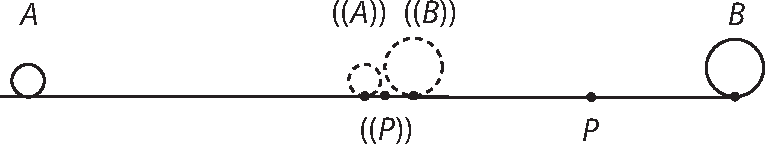
\includegraphics[width=0.66\textwidth]{%
gesamttex/edit_VIII,3/images/LH_37_05_162v_d1b.pdf%
}} 
\vspace{0.5em}
\centerline{%
\lbrack\textit{Fig.~1b, gültige Fassung}\rbrack%
}
% \newpage%
%
\vspace{1.5em} %%%%%%%%% Diagramm 2, gestr.
\centerline{%
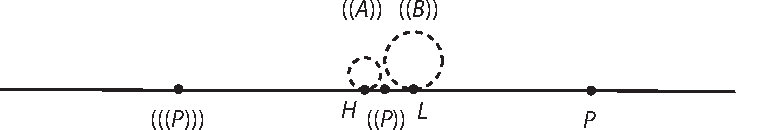
\includegraphics[width=0.66\textwidth]{%
gesamttex/edit_VIII,3/images/LH_37_05_162v_d2.pdf%
}} 
\vspace{0.5em}
\centerline{%
\lbrack\textit{Fig.~2, gestr.}\rbrack%
}
\newpage%
%
%%%%%%%% Diagramm 3
\centerline{%
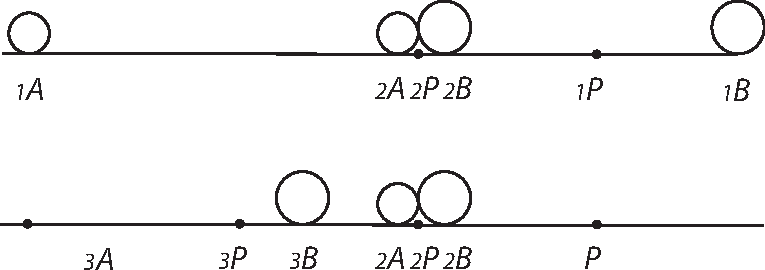
\includegraphics[width=0.66\textwidth]{%
gesamttex/edit_VIII,3/images/LH_37_05_162v_d3.pdf%
}} 
\vspace{0.5em}
\centerline{%
\lbrack\textit{Fig.~3}\rbrack%
}
% \newpage%
\vspace{1.5em}
%
\pstart 
\noindent
Corporum \textit{A}, \textit{B} distantia \edtext{prima \textit{AB}}{%
\lemma{prima}%
\Bfootnote{%
\textit{(1)}~$d\, \sqcap$ %
\textit{(2)}~\textit{AB} %
\textit{(3)}~\textit{DE} %
\textit{(4)}~\textit{AB}~
\textit{L}%
}}
%
sit \textit{d}. %
Celeritas\protect\index{Sachverzeichnis}{celeritas} qua 
%
\edtext{movetur \textit{A} seu $A{\scriptstyle \textit{2}}A$}{%
\lemma{movetur \textit{A}}%
\Bfootnote{%
\textit{(1)}~seu 
\textit{(a)}~\textit{A}(\textit{A}) %
\textit{(b)}~$A{\scriptstyle \textit{2}}A$ % %
\textit{(2)}~seu $A{\scriptstyle \textit{2}}A$~\textit{L}%
}}
%
sit \textit{c}. Celeritas qua movetur \textit{B}
%
\edtext{seu $B{\scriptstyle \textit{2}}B$}{\lemma{}\Bfootnote{seu $B{\scriptstyle \textit{2}}B$ \textit{erg.}~\textit{L}}}
\rule[0cm]{0mm}{12pt}%
\edtext{sit \textit{v}. Ergo}{\lemma{sit \textit{v}.}
  \Bfootnote{\textit{(1)}~Celeritas inquam id est rectae transcursae \textit{a} designant \textit{c}, \textit{(2)}~Ergo~\textit{L}}} 
%
$\overset%
{\displaystyle A{\scriptstyle \textit{2}}A}{% Oben
{\textso{DF}}}$
\textso{ad}
$\overset%
{\displaystyle B{\scriptstyle \textit{2}}B}{% Oben
{\textso{EG}}}$
\textso{ut \textit{c} ad \textit{v}.}
%
Centrum gravitatis%
\protect\index{Sachverzeichnis}{centrum gravitatis} corporum in primo situ \textit{A}, \textit{B} sit \textit{P}, 
%
eritque $\underset{\displaystyle b}{AP}$ ad $ \underset{\displaystyle a}{PB}$, ut \textit{b} ad \textit{a}.\
%
posito \textit{a} et \textit{b} 
\edtext{repraesentare soliditatem%
\protect\index{Sachverzeichnis}{soliditas}}{\lemma{repraesentare}
   \Bfootnote{\textit{(1)}~molem \textit{(2)}~soliditatem~\textit{L}}}  
%
seu %
pondus\protect\index{Sachverzeichnis}{pondus} corporum \textit{A}.\ \textit{B}. Translatis corporibus ex \textit{A}.\ \textit{B}.\ in (\textit{A}).\ (\textit{B}) 
\rule[0cm]{0mm}{12pt} 
quaeratur punctum \textit{P}
%
%
\edlabel{37_05_162v_8a}%
\edtext{}{% A-Footnote Hilfsrechnung
{\xxref%
{37_05_162v_8a}{37_05_162v_8b}}%
\lemma{}%
\Afootnote{%
\textit{Hilfsrechnung am oberen Blattrand}: 
$\displaystyle\dfrac{a+b-c-v}{a+b} \,\sqcap \dfrac{F(P)}{b}\,\sqcap \dfrac{(P)G}{a}$%
}}%
tale \edtext{ut sint $\underset{\displaystyle{a+b}}{AB}$, $\underset{\displaystyle{b}}{AP}$, $\underset{\displaystyle{a}\protect\vphantom{b}}{PB}$}{\lemma{ut}\Bfootnote{%
\textit{(1)}~sit %
\textit{(2)}~sint 
\textit{(a)}~$\protect\underset{\displaystyle{a+b}}{DE}$, $\protect\underset{\displaystyle{b}}{DP}$, $\protect\underset{\displaystyle{a}\protect\vphantom{b}}{PE}$
\textit{(b)}~$\protect\underset{\displaystyle{a+b}}{AB}$, $\protect\underset{\displaystyle{b}}{AP}$, $\protect\underset{\displaystyle{a}\protect\vphantom{b}}{PB}$~\textit{L}}}
%  
proportionales 
%
\edtext{ipsis $\underset{\displaystyle{a+b-c-v}}{{\scriptstyle \textit{2}}A {\scriptstyle \textit{2}}B}$\,, 
$\underset{\displaystyle{b-b\frac{c+v}{a+b}}}{{\scriptstyle \textit{2}}A {\scriptstyle \textit{2}}P}$\,,
$\underset{\displaystyle{a-a\frac{c+v}{a+b}}}{{\scriptstyle \textit{2}}B {\scriptstyle \textit{2}}P}$\,.}{%
\lemma{ipsis}%
\Bfootnote{%
\textit{(1)}~ $\protect\underset{\displaystyle{a+b-c-v}}{\textit{FG}}$\,, 
$\protect\underset{\displaystyle{b-b\frac{c+v}{a+b}}}{\textit{F}(\textit{P})}$\,,
\textbar\ $\protect\underset{\displaystyle{a-a\frac{c+v}{a+b}}}{(\textit{P})G}$\,. \textit{streicht Hrsg.}~\textbar\ %
\textit{(2)}~$\protect\underset{\displaystyle{a+b-c-v}}{{\scriptstyle \textit{2}}A {\scriptstyle \textit{2}}B}$\,, 
$\protect\underset{\displaystyle{b-b\frac{c+v}{a+b}}}{{\scriptstyle \textit{2}}A {\scriptstyle \textit{2}}P}$\,,
$\protect\underset{\displaystyle{a-a\frac{c+v}{a+b}}}{{\scriptstyle \textit{2}}B {\scriptstyle \textit{2}}P}$\,.~\textit{L}%
}}%
\edlabel{37_05_162v_8b}
%
\edtext{
Et $A{\scriptstyle \textit{2}}P \,\sqcap \underset{\displaystyle{c\protect\vphantom{\frac{a}{a}}}}{A {\scriptstyle \textit{2}}A} % 
\underset{\displaystyle{+\protect\vphantom{\frac{a}{a}}}}{+} %
\underset{\displaystyle{b-b\frac{c+v}{a+b}}}{{\scriptstyle \textit{2}}A {\scriptstyle \textit{2}}P}$ quod
}%
{\lemma{Et}%
\Bfootnote{%
\textit{(1)}~\textit{P}(\textit{P}) %
\textit{(2)}~\textit{D}(\textit{P}) %
\textit{(3)}~$A{\scriptstyle2}P \,\sqcap$ %
\textit{(a)}~$\protect\underset{\displaystyle{c\protect\vphantom{\frac{a}{a}}}}{DF} % 
\protect\underset{\displaystyle{+\protect\vphantom{\frac{a}{a}}}}{+} %
\protect\underset{\displaystyle{b-b\frac{c+v}{a+b}}}{F(P)}$
\textit{(b)}~$\protect\underset{\displaystyle{c\protect\vphantom{\frac{a}{a}}}}{A {\scriptstyle \textit{2}}A} % 
\protect\underset{\displaystyle{+\protect\vphantom{\frac{a}{a}}}}{+} %
\protect\underset{\displaystyle{b-b\frac{c+v}{a+b}}}{{\scriptstyle \textit{2}}A {\scriptstyle \textit{2}}P}$ %
\textit{(aa)}~quae quantitas si %
\textit{(bb)}~quod ~\textit{L}%
}}
%
\edtext{si  \textit{A{\scriptsize2}P} detrahatur a \textit{AP},}{\lemma{si}\Bfootnote{\textit{(1)}~(\textit{P})\textit{P} \textit{str.\ Hrsg.} \textit{(2)}~\textit{A{\scriptsize2}P} 
detrahatur a \textit{(a)}~\textit{DP} \textit{(b)}~\textit{AP},~\textit{L}}} 
%
\rule[0cm]{0mm}{10pt}%
seu a \textit{b}.\ 
%
\rule[0cm]{0mm}{20pt}%
\edtext{habebitur $P{\scriptstyle \textit{2}}P}{%
\lemma{habebitur}%
\Bfootnote{%
\textit{(1)}~\textit{P}(\textit{P}) %
\textit{(2)}~$P{\scriptstyle \textit{2}}P$~\textit{L}%
}}%
 \,\sqcap \ovalbox{$+b,$} -c \;\ovalbox{\!$-b\vphantom,$} + b\,\dfrac{c+v}{a+b}\, \sqcap \dfrac{-ac\; {\ovalbox{$-bc$}}\;{\ovalbox{$+bc$}}+bv}{a+b}$ 
%
\edlabel{37_05_162v_9a}%		zwecks Referenz
seu
%
\edtext{erit $P{\scriptstyle \textit{2}}P}{%
\lemma{erit}%
\Bfootnote{%
\textit{(1)}~\textit{P}(\textit{P}) %
\textit{(2)}~$P{\scriptstyle \textit{2}}P$ 
\textit{L}%
}}%
 \,\sqcap \dfrac{-ac+bv}{a+b}$.
 \pend
 \newpage
 \pstart
 \noindent Unde theorema: si duo corpora in eadem 
%
\edtext{recta sibi obviam eant erit productum sub %
celeritate centri gravitatis\protect\index{Sachverzeichnis}{celeritas centri gravitatis} in summam corporum,%
\protect\index{Sachverzeichnis}{productum celeritatis centri gravitatis in summa corporum} aequale differentiae productorum}{\lemma{recta}\Bfootnote{%
\textit{(1)}~moveantur, progressus eo 
\textit{(2)}~ad se invicem 
\textit{(3)}~sibi 
\textit{(a)}~accedant 
\textit{(b)}~obviam eant erit
\textit{(aa)}~rectangulum sub progressu centri gravitatis in %
\textit{(aaa)}~distantiam primam
\textit{(bbb)}~summam corporum, aequale differentiae %
\textit{(aaaa)}~sub corporum %
\textit{(bbbb)}~rectangulorum singulorum     
\textit{(bb)}~productum \lbrack...\rbrack\ productorum~\textit{L}}}
%
ex singulis corporibus in suas 
\edtext{celeritates.%
\protect\index{Sachverzeichnis}{productum corporis in suam celeritatem} Si ferantur}{\lemma{celeritates.}
  \Bfootnote{\textit{(1)}~Si non accedant, sed recedant, vel si 
  \textit{(2)}~Si \textit{(a)}~non \textit{(b)}~ferantur~\textit{L}}} 
in eadem recta ad easdem partes erit aequale summae.\edlabel{37_05_162v_9b} 
\pend
%
\pstart Hinc patet quamdiu corporum
in eadem recta motorum %
celeritas\protect\index{Sachverzeichnis}{celeritas} eadem est, eandem etiam esse celeritatem 
\edtext{centri.%
\protect\index{Sachverzeichnis}{celeritas centri} Cum}{\lemma{centri.}\Bfootnote{\textit{(1)}~(Video tamen corpora in diversis rectis unita produci suo quodammodo potest.) \textit{(2)}~Cum~\textit{L}}} 
enim magnitudo sit invariabilis, tam singulorum quam summae patet celeritatem
centri%
\protect\index{Sachverzeichnis}{celeritas centri} non nisi mutatione celeritatis%
\protect\index{Sachverzeichnis}{mutatio celeritatis} in corporibus mutari posse.
\pend
%
\pstart
Momento concursus%
\protect\index{Sachverzeichnis}{momentum concursus} sit %
centrum gravitatis\protect\index{Sachverzeichnis}{centrum gravitatis} \textit{{\scriptsize2}P}, 
%<?>
%<?>
corporibus \edtext{positis in \textit{{\scriptsize2}A}\lbrack,\rbrack\ \textit{{\scriptsize2}B}}{%
\lemma{positis in}%
\Bfootnote{%
\textit{(1)}~((\textit{A}))((\textit{B})) %
\textit{(2)}~\textit{{\scriptsize2}A}\lbrack,\rbrack\ \textit{{\scriptsize2}B}~\textit{L}%
}}
%
seque tangentibus. 
%
Quoniam %
\edtext{autem ostendimus}{\lemma{autem}\Bfootnote{\textit{(1)}~poni \textit{(2)}~ostendimus~\textit{L}}} 
centrum corporum uniformi celeritate procedere usque ad concursum, supponimus vero idem contingere
%<?>
post concursum,%
\protect\index{Sachverzeichnis}{concursus} hinc tempore quo \textit{P} 
%
\edtext{pervenit in \textit{{\scriptsize2}P}}{%
\lemma{pervenit in}%
\Bfootnote{%
\textit{(1)}~((\textit{P})) %
\textit{(2)}~\textit{{\scriptsize2}P}~\textit{L}%
}}
%
ante concursum%
\protect\index{Sachverzeichnis}{concursus} etiam post concursum 
%
\edtext{perveniet in \textit{{\scriptsize3}P}.}{%
\lemma{perveniet in}%
\Bfootnote{%
\textit{(1)}~(((\textit{P}))) %
\textit{(2)}~\textit{{\scriptsize3}P}~\textit{L}%
}}
%
\edtext{Eruntque \textit{P{\scriptsize2}P}, et \textit{{\scriptsize2}P{\scriptsize3}P}}{%
\lemma{Eruntque}%
\Bfootnote{%
\textit{(1)}~\textit{P}((\textit{P})) et ((\textit{P}))(((\textit{P}))) %
\textit{(2)}~\textit{P{\scriptsize2}P}, et \textit{{\scriptsize2}P{\scriptsize3}P}~\textit{L}%
}}
%
\edtext{aequales. Habetur autem recta \textit{P{\scriptsize2}P} vel \textit{{\scriptsize2}P{\scriptsize3}P}
hoc modo\!
$\protect\underset%
{\displaystyle \phantom(\text{vel \textit{{\scriptsize2}P{\scriptsize3}P}}\phantom)}% Unten
{\phantom(\text{\textit{P{\scriptsize2}P}}\phantom)} %
\sqcap$}%
{\lemma{aequales.}\Bfootnote{%
\textit{(1)}~Hinc jam habebitur recta %
\textit{(a)}~\textit{P}(\protect\vphantom)(\protect\vphantom)\textit{P} \textit{(b)}~(\protect\vphantom)(\protect\vphantom)\textit{P} \textit{(c)}~\textit{P} \textit{(2)}~Habetur autem recta %
\textit{(a)}~\textit{P}((\textit{P})) \textbar\ recta \textit{streicht Hrsg.}~\textbar\ %
((\textit{P}))(((\textit{P}))) hoc modo 
$\protect\underset%
{\displaystyle \text{vel ((\textit{P}))(((\textit{P})))}}% Unten
{\text{\textit{P}((\textit{P}))}}%
\sqcap \dfrac{-ac+bv}{\hphantom{}}$ %
\textit{(b)}~\textit{P{\scriptsize2}P} vel \textit{{\scriptsize2}P{\scriptsize3}P} \textbar\ \textit{{\scriptsize2}P} \textit{streicht Hrsg.}~\textbar\ %
 hoc modo %
$\protect\underset%
{\displaystyle \phantom(\text{vel \textit{{\scriptsize2}P{\scriptsize3}P}}\phantom)}% Unten
{\phantom(\text{\textit{P{\scriptsize2}P}}\phantom)}%
\sqcap \;$
\textit{L}%
}}
$\dfrac{-ac+bv}{a+b}$,
%
\rule[0cm]{0mm}{16pt}%
\edtext{id est $\dfrac{-PB,A{\scriptstyle \textit{2}}A,,+PA,B{\scriptstyle \textit{2}}B}{AB}$ at idem
${\scriptstyle \textit{3}}P{\scriptstyle \textit{2}}P\, \sqcap 
\dfrac{-{\scriptstyle \textit{3}}P {\scriptstyle \textit{3}}B, {\scriptstyle \textit{3}}A {\scriptstyle \textit{2}}A,,+{\scriptstyle \textit{3}}P {\scriptstyle \textit{3}}A, {\scriptstyle \textit{3}}B {\scriptstyle \textit{2}}B}{{\scriptstyle \textit{3}}A {\scriptstyle \textit{3}}B}$, 
vel}{%
\lemma{id est \lbrack...\rbrack\ vel}%
\Cfootnote{%
Leibniz verwendet hier das Komma als Multiplikationszeichen.%
}}
%
\rule[0cm]{0mm}{16pt}%
$\dfrac{-\alpha\gamma+\beta\protect\rotatebox{0}{$\downpropto$}}{\alpha+\beta}$ 
\pend %ponendo scilicet...
%
\pstart\noindent
\rule[0cm]{0pt}{14pt}ponendo
\edtext{scilicet \textit{b} vel $\beta$ esse corporis \textit{A} vel \textit{{\scriptsize2}A} distantiam a}{%
\lemma{scilicet}\Bfootnote{%
\textit{(1)}~\textit{a} vel $\alpha$
\textit{(2)}~\textit{b} vel $\beta$ esse
\textit{(a)}~distantiam corporis \textit{A} a
\textit{(b)}~corporis \textit{A} vel \textit{{\scriptsize2}A} distantiam a~%
\textit{L}}} 
%
centro gravitatis\protect\index{Sachverzeichnis}{distantia a centro gravitatis} \textit{P} vel
%
\edlabel{37_05_162v_3a}%
\edtext{}{{\xxref{37_05_162v_3a}{37_05_162v_3b}}%
\lemma{\textit{{\scriptsize2}P}}%
\Bfootnote{%
\textit{(1)}~et \textbar\ \textit{c} vel \textit{gestr.} \textbar\ 
$\protect\underset%
{\protect\rotatebox{0}{$\downpropto$}}{% Unten
{\gamma}}$ 
esse celeritatem ipsius 
$\protect\underset%
{\displaystyle\textit{b}}{% Unten
{\textit{A}}}$
\textit{(2)}~\textit{b} vel $\beta$
\textit{(3)}~\textit{a} vel $\alpha$~\textit{L}}}%
\textit{{\scriptsize2}P}
%
\hphantom{ponendo scilicet} 
\textit{a} vel $\alpha$%
\edlabel{37_05_162v_3b}
%
\hphantom{esse}%
\newlength{\corporis}\settowidth{\corporis}{corporis}
\parbox[b][][b]{\corporis}{$\dotfill$}\hspace{1mm} $B$ vel \textit{{\scriptsize2}B}
\newlength{\distantiam}\settowidth{\distantiam}{distantiam a centro gravitatis \textit{P} vel \textit{{\scriptsize2}P}}%
\parbox[b][0 pt][b]{\distantiam}{$\dotfill$}
%\pend %et rursus...
%\newpage
%\pstart\noindent
et rursus \textit{c} vel $\gamma$ esse celeritatem ipsius 
\edtext{\textit{A} vel}{\lemma{\textit{A}}\Bfootnote{\textit{(1)}~qua pervenit \textit{(2)}~vel~\textit{L}}} 
\textit{{\scriptsize2}A} seu spatium quod trajecit 
\textit{A{\scriptsize2}A} vel \textit{{\scriptsize2}A{\scriptsize3}A}
%
\noindent\hphantom{et rursus} %
%\newlength{\mylengtha}\settowidth{\mylengtha}{\textit{c} vel $\gamma$.}%
%\parbox[b][][b]{\mylengtha} 
\hphantom{esse celeritatem ipsius}%
\textit{B} %
vel \textit{{\scriptsize2}B}%
\newlength{\spatium}\settowidth{\spatium}{seu spatium quod trajecit}
\parbox[b][][b]{\spatium}{$\dotfill$}
\textit{B{\scriptsize2}B} vel \textit{{\scriptsize2}B{\scriptsize3}B}.%
\pend
\newpage
%\rule[0cm]{20mm}{0cm}
%
\pstart
Habemus ergo aequationem unam: $\dfrac{-ac+bv}{a+b} \,\overset{(1)}\sqcap \dfrac{-\alpha\gamma+\beta\protect\rotatebox{0}{$\downpropto$}}{\alpha+\beta}$, sed habemus et alias aequationes nempe semper ratio
distantiarum a centro gravitatis%
\protect\index{Sachverzeichnis}{distantia a centro gravitatis}%
\protect\index{Sachverzeichnis}{ratio distantiarum a centro gravitatis} eadem, seu  $\dfrac{a}{b} \,\overset{(2)}\sqcap \dfrac{\alpha}{\beta}$. Ergo
$\dfrac{a+b}{\alpha+\beta} \,\overset{(3)}\sqcap %
\edtext{\dfrac{a}{\alpha}$. Ergo}
  {\lemma{$\dfrac{a}{\alpha}$.}\Bfootnote{\textit{(1)}~seu $\alpha + \beta \sqcap \overline{a+b} \dfrac{\alpha}{a}$ \textit{(2)}~Ergo~\textit{L}}} 
ex aequ.\ 1 e\textlangle t 3\textrangle\ junctis fiet: 
$\dfrac{-ac+bv}{-\alpha\gamma+\beta\protect\rotatebox{0}{$\downpropto$}} \,\overset{(4)}\sqcap \dfrac{a}{\alpha} \,\sqcap \dfrac{b}{\beta}$.
%
\rule[0cm]{0mm}{16pt}%
\edtext{Rursus}{\lemma{Rursus}\Bfootnote{\textit{(1)}~$+ ac + bv  \,\sqcap + \alpha\gamma+ $ \textit{(2)}~\textit{ac}~\textit{L}}} 
$ac + bv  \,\overset{(5)}\sqcap \alpha\gamma+\beta\protect\rotatebox{0}{$\downpropto$}$. 
%
\rule[0cm]{0mm}{10pt}%
Posito scilicet
quod eadem quantitas 
\edtext{potentiae%
\protect\index{Sachverzeichnis}{quantitas potentiae} supersit}{\lemma{potentiae}
  \Bfootnote{\textit{(1)}~inter \textit{(2)}~ante \textit{(3)}~supersit~\textit{L}}} 
post concursum quam ante, potentiae%
\protect\index{Sachverzeichnis}{potentia} enim sunt ut rectangula
\edtext{ex recta transcursa}{\lemma{ex}\Bfootnote{\textit{(1)}~celerita \textit{(2)}~spa \textit{(3)}~recta \textit{(a)}~concursa \textit{(b)}~transcursa~\textit{L}}} 
\edtext{in brachium%
\protect\index{Sachverzeichnis}{brachium}}{\lemma{in}\Bfootnote{\textit{(1)}~centrum \textit{(2)}~dis \textit{(3)}~brachium~\textit{L}}}
corporis oppositi. Quia \textit{c} recta transcursa significat celeritatem,%
\protect\index{Sachverzeichnis}{celeritas} 
\edtext{\textit{a}, brachium\protect\index{Sachverzeichnis}{brachium}}{\lemma{\textit{a},}\Bfootnote{\textit{(1)}~distantia corpo \textit{(2)}~brachium~\textit{L}}}
seu a centro distantia%
\protect\index{Sachverzeichnis}{distantia a centro} corporis oppositi significat ipsius corporis magnitudinem,%
\protect\index{Sachverzeichnis}{magnitudo corporis} (%
brachia\protect\index{Sachverzeichnis}{brachium} enim sunt reciproce ut corpora). Habemus ergo omnia lineis%
%
\edlabel{37_05_162v_4a}%
\edtext{}{% B-Footnote – "expressa. Ex"
{\xxref%
{37_05_162v_4a}{37_05_162v_4b}}%
\lemma{expressa.}%
\Bfootnote{%
\textit{(1)}~Hinc 
\textit{(a)}~si in aequ.\ 4 
\textit{(b)}~$a+b$  
\textit{(c)}~$\dfrac{ac+bv}{\alpha\gamma+\beta\protect\rotatebox{0}{$\downpropto$}} \,\protect\overset{(6)}\sqcap 1$.
Ergo si addatur aequ.\ 6 aequationi 4, fiet $\dfrac{{\protect\ovalbox{$+ac$}} +bv\, {\protect\ovalbox{\!$-ac$}} +bv}{\alpha\gamma+\beta\protect\rotatebox{0}{$\downpropto$}}\,\sqcap \dfrac{a+\alpha}{\alpha} \,\protect\overset{(7)}\sqcap \dfrac{2bv}{\alpha\gamma+\beta\protect\rotatebox{0}{$\downpropto$}}$
\textit{(aa)}~Eodemque jure
\textit{(bb)}~$\sqcap \,\dfrac{b+\beta}{\beta}$.
\textit{(aaa)}~Et reducendo $\dfrac{2b\beta\protect\rotatebox{0}{$\downpropto$}}{\hphantom{a}}$
\textit{(bbb)}~Eodemque jure $\dfrac{+\alpha\gamma+\beta\protect\rotatebox{0}{$\downpropto$}-\alpha\gamma+\beta\protect\rotatebox{0}{$\downpropto$}}
{\hphantom{a}}$
\textit{(2)}~$\protect\underset{\displaystyle ac+bv}{\protect\underbrace{2ac-ac+bv}}\,\sqcap
2ac + \dfrac{a}{\alpha}\protect\overline{\alpha\gamma+\beta\protect\rotatebox{0}{$\downpropto$}}\,\sqcap 
\protect\underset{{\displaystyle -a}\protect\vphantom{-\dfrac{a}{\alpha}}}{+\alpha}\gamma\protect\underset{-\dfrac{a}{\alpha}}{+1}\beta\protect\rotatebox{0}{$\downpropto$} $. 
Ergo $2ac\,\sqcap \protect\overline{1-\dfrac{a}{\alpha}}\beta\protect\rotatebox{0}{$\downpropto$}$
seu $2ac\,\sqcap \beta\protect\rotatebox{0}{$\downpropto$} - \dfrac{\beta}{\alpha}a\protect\rotatebox{0}{$\downpropto$}$. 
Et quia $\dfrac{\beta}{\alpha}\,\sqcap \dfrac{b}{a}$
erit $2ac \,\sqcap \beta\protect\rotatebox{0}{$\downpropto$} - b\protect\rotatebox{0}{$\downpropto$}$  
\textit{(a)}~seu $2ac \,\sqcap$
\textit{(b)}~rursus  $\protect\underset{{\displaystyle\alpha\gamma+\beta\protect\rotatebox{0}{$\downpropto$}}}{\protect\underbrace{2\alpha\gamma-\alpha\gamma+\beta\protect\rotatebox{0}{$\downpropto$}}}\,\sqcap 
2\alpha\gamma + \dfrac{\alpha}{a}-\protect\overline{ac+bv} \,\sqcap ac+bv$. Ergo
\textit{(3)}~Ex~\textit{L}}} 
%
expressa.
%
\pend
%
\pstart 
Ex%
\edlabel{37_05_162v_4b}
%
\rule[0cm]{0mm}{16pt}%
4.\ $\dfrac{-\alpha\gamma+\beta\protect\rotatebox{0}{$\downpropto$}}{\beta} \,\overset{(6)}\sqcap \dfrac{-ac+bv}{b}$ jam 
%
\edtext{$\dfrac{-\alpha\gamma}{\beta} \,\overset{(7)}\sqcap -\dfrac{a}{b}\gamma$ ex 2.}
{\lemma{$\dfrac{-\alpha\gamma}{\beta} \,\protect\overset{(7)}\sqcap -\dfrac{a}{b}\gamma$}\Bfootnote{\textit{(1)}~$+ \protect\rotatebox{0}{$\downpropto$} \,\sqcap \dfrac{-ac+bv}{b}$ 
\textit{(2)}~ ex 2.~\textit{L}}} 
%
Ergo ex 6.\ 7.\ erit $\dfrac{-a}{b}\gamma + \protect\rotatebox{0}{$\downpropto$} \,\overset{(8)}\sqcap \dfrac{-ac+bv}{b}$. 
%
\rule[0cm]{0mm}{16pt}%
Seu erit
$-a\gamma + b\protect\rotatebox{0}{$\downpropto$} \,\overset{(9)}\sqcap -ac+bv $
seu $ +a \smallfrown \underset{{\displaystyle -\gamma}}{+c} \,\overset{(10)}\sqcap 
+b\smallfrown \underset{{\displaystyle -\protect\rotatebox{0}{$\downpropto$}}}{+v}$.
\edlabel{37_05_162v_10a}%	zwecks Referenz
Ergo erit $\dfrac{a}{b} \; \overset{(11)}\sqcap $
\edtext{$\dfrac{v-\protect\rotatebox{0}{$\downpropto$}}{c-\gamma}$ quod ex solis aequationibus 1.\ et 2.\ sequitur. Mutationes}{\lemma{}
\Bfootnote{$\protect\dfrac{v-\protect\rotatebox{0}{$\downpropto$}}{c-\gamma}$ \textbar\ quod \lbrack...\rbrack\ sequitur \textit{erg.} \ \textbar \ 
\textit{(1)}~Ut corpora ita differentiae celeritatum \textit{(2)}~Mutationes~\textit{L}}}
%
\rule[0cm]{0mm}{10pt}%
celeritatum%
\protect\index{Sachverzeichnis}{mutatio celeritatis} sunt ut corpora 
%
\edtext{reciproce. Hoc theorema substitui potest pro altero de gravitatis centro.\edlabel{37_05_162v_10b}%
\protect\index{Sachverzeichnis}{theorema de centro gravitatis}}{\lemma{}
\Bfootnote{reciproce. \lbrack...\rbrack\ de \textit{(1)}~mutatis \textit{(2)}~gravitatis centro. \textit{erg.}~\textit{L}}} 
\pend
\newpage
%
\pstart 
Similiter \rule[0cm]{0mm}{16pt}%
$\dfrac{-\alpha\gamma+\beta\protect\rotatebox{0}{$\downpropto$}}{\alpha} \,\sqcap \dfrac{-ac+bv}{a} \,\sqcap
-\gamma + \dfrac{b}{a}\protect\rotatebox{0}{$\downpropto$}$. Ergo $-ac+bv \,\sqcap -\gamma a + b\protect\rotatebox{0}{$\downpropto$}$, ut ante.
\pend
%
\pstart 
Si ad aequationem 9.\ addatur aequ.\ 5 fiet: 
$\genfrac{}{}{0pt}{0}{-a\gamma + b\protect\rotatebox{0}{$\downpropto$}}{+\alpha\gamma + \beta\protect\rotatebox{0}{$\downpropto$}} \,\sqcap
\,\ovalbox{$\displaystyle\efrac{-ac}{+ac}$} \, \displaystyle\efrac{+bv}{+bv}$.
Ergo  $ \gamma \smallfrown \underset{{\displaystyle +\alpha}}{-a},, 
+\protect\rotatebox{0}{$\downpropto$}\smallfrown \underset{{\displaystyle +\beta}}{+b}\,\overset{(12)}\sqcap 2bv$
rursus $\genfrac{}{}{0pt}{0}{-a\gamma + b\protect\rotatebox{0}{$\downpropto$}}{-\alpha\gamma - \beta\protect\rotatebox{0}{$\downpropto$}} \,\sqcap
\displaystyle\efrac{-ac}{-ac}\; \ovalbox{$\displaystyle\efrac{+bv}{-bv}$} $\,.
Ergo  $ -\gamma \smallfrown \underset{{\displaystyle \alpha}}{a} 
+\protect\rotatebox{0}{$\downpropto$}\smallfrown \underset{{\displaystyle -\beta}}{+b}\,\overset{(13)}\sqcap -2ac$ addendo 
aequationem 12 et 13, fiet:
$-\cancel 2 \gamma\alpha + \cancel 2 \protect\rotatebox{0}{$\downpropto$} b \,\sqcap \cancel 2 bv - \cancel 2 ac$.
Seu $\underset{-\protect\rotatebox{0}{$\downpropto$}}{+v}\smallfrown b \,\overset{(14)}\sqcap ac-\alpha\gamma
\,\overset{(15)\; \textrm{per}\; 10}\sqcap ac-a\gamma$. Ergo ex 15.\ fiet $\alpha \,\overset{(16)}\sqcap a$.
Ergo et
%
\edlabel{37_05_162v_5a}%
\edtext{}{% NEUER ABSATZ UND VARIANTEN – Rechnung 17
{\xxref%
{37_05_162v_5a}{37_05_162v_5b}}%
\lemma{$\beta \,\protect\overset{(17)}\sqcap b$.}
\Bfootnote{\textit{(1)}~Ergo et $c-\gamma \,\protect\overset{(18)}\sqcap v-\protect\rotatebox{0}{$\downpropto$}$.
Ergo et  \textit{(a)}~$c-v\;\sqcap$ \textit{(b)}~$\gamma-\protect\rotatebox{0}{$\downpropto$} \,\protect\overset{(19)}\sqcap c-v$. 
\textit{(2)}~Ergo~\textit{L}}}%
$\beta \,\overset{(17)}\sqcap b$.
\pend
%
\pstart
Ergo%
\edlabel{37_05_162v_5b}
%
\rule[0cm]{0mm}{16pt}%
$-ac+bv \,\overset{(18)}\sqcap -\alpha\gamma + b\protect\rotatebox{0}{$\downpropto$}$. 
Vel $-ac+bv \,\sqcap -a\gamma + b\protect\rotatebox{0}{$\downpropto$}$. Seu 
$\underset{{\displaystyle -\protect\rotatebox{0}{$\downpropto$}}}{+v}\smallfrown b \,\sqcap 
\underset{{\displaystyle -\gamma}}{+c}\smallfrown a$.
Prorsus ut 9.\ 10.\ 11. 
Rursus: ex 5 fiet $ac+bv\,\overset{(19)}\sqcap \alpha\gamma + b\protect\rotatebox{0}{$\downpropto$}$. Addantur 9 et 19 fiet: 
$2bv \,\sqcap 2b\protect\rotatebox{0}{$\downpropto$}$. Unde fiet $\protect\rotatebox{0}{$\downpropto$} \sqcap v$. Quod est absurdum, ergo 
errorem alicubi in calculo latere necesse est.\edlabel{37_05_162v_11b}
\pend
%%%%%%%
%
\vspace{0.5em} % evtl. entfernen
%
\pstart
\noindent
\lbrack%
\edlabel{37_05_162v_12a}%
\textit{Zweiter Anlauf:}\rbrack % Zweiter Anlauf, bis Ende 162~v\textsuperscript{o}; ggf. abbrechend??}
\pend
%%%%%%
%
\vspace{2.0em} %%%%%%%%% Diagramm 4
\centerline{%
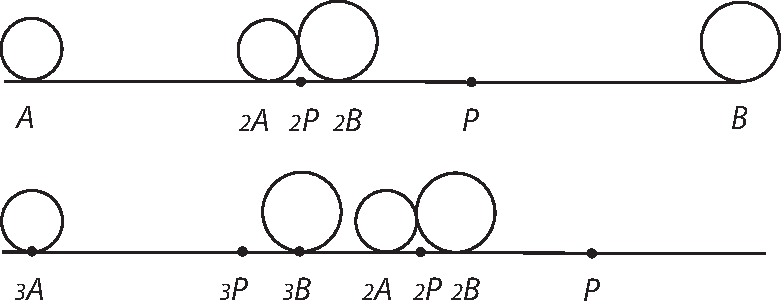
\includegraphics[width=0.66\textwidth]{%
gesamttex/edit_VIII,3/images/LH_37_05_162v_d4.pdf%
}} 
\vspace{0.5em}
\centerline{%
\lbrack\textit{Fig.~4}\rbrack%
}
\newpage%
%\vspace{1.5em}
%
\pstart
\noindent
Corpora \textit{A}, \textit{B}.\ concurrunt celeritatibus \textit{A{\scriptsize2}A}, \textit{B{\scriptsize2}B}. 
%
%
\edlabel{37_05_162v_6a}%
\edtext{}{% C-Footnote Klein- und Großschreibung
{\xxref%
{37_05_162v_6a}{37_05_162v_6b}}%
\lemma{Centrum \lbrack...\rbrack\ \textit{{\scriptsize3}}\textit{p}}%
\Cfootnote{%
Leibniz wechselt in der Bezeichnung des Schwerpunkts zwischen \textit{P} und \textit{p}.}}%
%
Centrum gravitatis%
\protect\index{Sachverzeichnis}{centrum gravitatis} eorum in primo situ est \textit{P}.\ ita ut sit \textit{AP} ad 
\textit{B}\textit{p}
ut \textit{B} corpus ad \textit{A} corpus. Centrum gravitatis in situ secundo seu concursu est 
\edtext{\textit{{\scriptsize2}}\lbrack\textit{P}\rbrack.}{\lemma{}\Bfootnote{\textit{P} \textit{\ erg. Hrsg.}}} 
Quoniam autem %
centrum gravitatis\protect\index{Sachverzeichnis}{centrum gravitatis} eadem semper 
\edtext{\lbrack celeritate\rbrack}{\lemma{}\Bfootnote{gravitate \textit{\ L ändert Hrsg.}}}
procedere%
\protect\index{Sachverzeichnis}{centrum gravitatis eadem semper celeritate procedens} supponimus, ideo tempore
e\textlangle o\textrangle dem 
quo ex 
\textit{p} pervenit in \textit{{\scriptsize2}}\textit{p}, idem centrum gravitatis ex \textit{{\scriptsize2}}\textit{p} perveniet in \textit{{\scriptsize3}}\textit{p}, ita ut sit \textit{{\scriptsize2}}\textit{p}\textit{{\scriptsize3}}\textit{p} aequalis ipsi \textit{p}\textit{{\scriptsize2}}\textit{p}. Datur ergo punctum \textit{{\scriptsize3}}\textit{p},\edlabel{37_05_162v_6b}
quaeruntur
puncta ${\scriptstyle \textit{3}}A$.\ ${\scriptstyle \textit{3}}B$.\ seu situs corporum concurrentium post concursum.%
\protect\index{Sachverzeichnis}{concursus} 
Sc\textlangle im\textrangle us
autem esse \textit{{\scriptsize3}A{\scriptsize3}P} ad \textit{{\scriptsize3}B{\scriptsize3}P}, ut corpus \textit{B} ad corpus 
\edtext{\textit{A} seu}{\lemma{\textit{A}}\Bfootnote{\textit{(1)}~. Item \textit{(a)}~scimus \textit{(b)}~ponimus esse 
\textit{(2)}~seu~\textit{L}}}
ut \textit{AP} ad \textit{BP}.
Item supponimus esse 
%<cele>
eandem potentiam%
\protect\index{Sachverzeichnis}{potentia} quae ante, seu 
sum\textlangle ma\textrangle\
celeritatum in corpora, sive ${\scriptstyle \textit{2}}A {\scriptstyle \textit{3}}A \text{ in } BP + {\scriptstyle \textit{2}}B {\scriptstyle \textit{3}}B \text{ in } AP \,\overset{(1)}\sqcap A {\scriptstyle \textit{2}}A \text{ in } BP + B{\scriptstyle \textit{2}}B \text{ in } AP$. Est autem ${\scriptstyle \textit{2}}A {\scriptstyle \textit{3}}A \,\overset{(2)}\sqcap {\scriptstyle \textit{2}}A {\scriptstyle \textit{3}}P + {\scriptstyle \textit{3}}A {\scriptstyle \textit{3}}P$ et
${\scriptstyle \textit{2}}B {\scriptstyle \textit{3}}B \,\overset{(3)}\sqcap {\scriptstyle \textit{2}}B {\scriptstyle \textit{3}}P - 
% 
\edtext{{\scriptstyle \textit{3}}B {\scriptstyle \textit{3}}P$ et ut}%
{\lemma{${\scriptstyle \textit{3}}B {\scriptstyle \textit{3}}P$ et}%
\Bfootnote{\textit{(1)}~ex sup \textit{(2)}~ut~\textit{L}}} 
%
\rule[0cm]{0mm}{16pt}%
dixi ex natura centri ${\scriptstyle \textit{3}}A {\scriptstyle \textit{3}}P \text{ in } BP \,\overset{(4)}\sqcap {\scriptstyle \textit{3}}B {\scriptstyle \textit{3}}P \text{ in } AP$. In aequ.\ 1 pro \textit{{\scriptsize2}A{\scriptsize3}A} et \textit{{\scriptsize2}B{\scriptsize3}B} substituendo eorum valores ex aequ.\ 2.\ 3.\ fiet 
\edtext{${\scriptstyle \textit{2}}A {\scriptstyle \textit{3}}P \smallfrown BP,,$}{%
\lemma{}%
\Bfootnote{%
${\scriptstyle \textit{2}}A {\scriptstyle \textit{3}}P \smallfrown $ \textbar\ in \textit{streicht Hrsg.}~\textbar\ %
 $BP,,$~\textit{L}%
}}
$\ovalbox{$\vphantom{0}+ {\scriptstyle \textit{3}}A {\scriptstyle \textit{3}}P \smallfrown BP$}\, + {\scriptstyle \textit{2}}B {\scriptstyle \textit{3}}P
\smallfrown AP \,
{\ovalbox{$\underset{\displaystyle-{\scriptstyle \textit{3}}A {\scriptstyle \textit{3}}P \smallfrown BP \text{ per }4}{\underbrace{
\vphantom{0}- {\scriptstyle \textit{3}}B {\scriptstyle \textit{3}}P \smallfrown AP}}$}} \,\overset{(5)}\sqcap
A {\scriptstyle \textit{2}}A \text{ in } BP + B {\scriptstyle \textit{2}}B \text{ in } AP$.\pend
%
\pstart
${\scriptstyle \textit{2}}A {\scriptstyle \textit{3}}A\smallfrown BP, + {\scriptstyle \textit{2}}B {\scriptstyle \textit{3}}P \smallfrown AP \,\sqcap\vphantom{0}$\!
\rule[0cm]{0mm}{16pt}%
datae quantitati \textit{d}. Rursus 
${\scriptstyle \textit{2}}A {\scriptstyle \textit{3}}A - {\scriptstyle \textit{2}}A {\scriptstyle \textit{3}}P$ ad 
${\scriptstyle \textit{2}}B {\scriptstyle \textit{3}}P - {\scriptstyle \textit{2}}B {\scriptstyle \textit{3}}B$, ut \textit{AP} ad \textit{BP}. 
%
%
\edlabel{37_05_162v_7a}%
\edtext{}{% C-Footnote – Multiplikationszeichen
{\xxref%
{37_05_162v_7a}{37_05_162v_7b}}%
\lemma{Unde \lbrack...\rbrack\  \protect\ovalbox{\textit{BP}}\,}%
\Cfootnote{%
Leibniz verwendet hier das Komma als Multiplikationszeichen, neben dem üblicheren Zeichen $\smallfrown$\,.%
}}%
%
Unde ex hac analogia aequatio: 
${\scriptstyle \textit{2}}A {\scriptstyle \textit{3}}A,BP - {\scriptstyle \textit{2}}A {\scriptstyle \textit{3}}P,BP \,\sqcap
{\scriptstyle \textit{2}}B {\scriptstyle \textit{3}}P,AP,, - {\scriptstyle \textit{2}}B {\scriptstyle \textit{3}}B,AP$.
\pend
%
\pstart
Ex aequ.\ 5 
\rule[0cm]{0mm}{16pt}%
fiet $\displaystyle\dfrac{A {\scriptstyle \textit{2}}A - {\scriptstyle \textit{2}}A {\scriptstyle \textit{3}}P}
{{\scriptstyle \textit{2}}B {\scriptstyle \textit{3}}P - B {\scriptstyle \textit{2}}B}\,\sqcap \dfrac{AP}{BP}$. 
 ${\scriptstyle \textit{2}}B {\scriptstyle \textit{3}}P \,\sqcap {\scriptstyle \textit{2}}A {\scriptstyle \textit{3}}P + {\scriptstyle \textit{2}}A {\scriptstyle \textit{2}}B$.
Ergo fiet
$\displaystyle A {\scriptstyle \textit{2}}A,BP, - {\scriptstyle \textit{2}}A {\scriptstyle \textit{3}}P,BP\,\sqcap  
\underset{\displaystyle {\scriptstyle \textit{2}}A {\scriptstyle \textit{2}}\edlabel{37_05_162v_1a}\lbrack B\rbrack\edlabel{37_05_162v_1b}}{{\scriptstyle \textit{2}}A {\scriptstyle \textit{3}}P},AP,,-B{\scriptstyle \textit{2}}%
\langle B,AP.\rangle$%
\rule[0cm]{0mm}{12pt}%
\edtext{}{{\xxref{37_05_162v_1a}{37_05_162v_1b}}{\lemma{\textit{P}}\Bfootnote{\textit{L \ ändert Hrsg.}}}}
\pend
\pstart\noindent
Ergo ${\scriptstyle \textit{2}}A {\scriptstyle \textit{3}}P\,\sqcap
\dfrac{A {\scriptstyle \textit{2}}A,BP,, - {\scriptstyle \textit{2}}A {\scriptstyle \textit{2}}\edlabel{37_05_162v_2a}\lbrack B\rbrack\edlabel{37_05_162v_2b},AP,,+B{\scriptstyle \textit{2}}B,AP}
{\text{\textlangle} AP+\text{\textrangle} BP}$%
\edtext{}{{\xxref{37_05_162v_2a}{37_05_162v_2b}}{\lemma{}\Bfootnote{\textit{P}\textit{\ L \ ändert Hrsg.}}}}.
\pend
\pstart\noindent
Et\; $\underbrace{{\scriptstyle \textit{2}}A {\scriptstyle \textit{3}}P+{\scriptstyle \textit{2}}A {\scriptstyle \textit{2}}P}_{\displaystyle\langle{\scriptstyle \textit{2}}P {\scriptstyle \textit{3}}P\rangle}
\;\sqcap\; \langle A {\scriptstyle \textit{2}}A,\rangle BP,,$
\ovalbox{$-{\scriptstyle \textit{2}}A {\scriptstyle \textit{2}}B,AP,,$}
$+B{\scriptstyle \textit{2}}B,AP,,+$
\textlangle\textendash\textrangle\;\ovalbox{\textit{AP}}%
\edlabel{37_05_162v_7b}%
\rule[0cm]{0mm}{16pt}
\quad\lbrack\textit{Rechnung bricht ab.}\rbrack%
\edlabel{37_05_162v_12b}
\pend
\count\Bfootins=1200%
\count\Afootins=1200%
\count\Cfootins=1200
